% =============================================================================
% IEEE Conference Paper — Ultra-Light LLM Benchmarking
% Upload to Overleaf as main.tex and compile with pdfLaTeX
% =============================================================================
\documentclass[conference]{IEEEtran}
\IEEEoverridecommandlockouts

\usepackage{cite}
\usepackage{amsmath,amssymb,amsfonts}
\usepackage{algorithmic}
\usepackage{graphicx}
\usepackage{textcomp}
\usepackage{xcolor}
\usepackage{booktabs}
\usepackage{multirow}
\usepackage{colortbl}
\usepackage{url}
\usepackage{hyperref}
\usepackage{pgfplots}
\pgfplotsset{compat=1.18}
\usepackage{tikz}

\definecolor{darkgreen}{HTML}{2A7D6F}
\definecolor{darkred}{HTML}{B23030}
\definecolor{lightyellow}{HTML}{FFF8E1}
\definecolor{lightgreen}{HTML}{E8F4EA}

\hypersetup{
  colorlinks=true,
  linkcolor=black,
  citecolor=blue,
  urlcolor=blue
}

\def\BibTeX{{\rm B\kern-.05em{\sc i\kern-.025em b}\kern-.08em
    T\kern-.1667em\lower.7ex\hbox{E}\kern-.125emX}}

\begin{document}

\title{Benchmarking Ultra-Light Language Models\\ for Edge Deployment: A Cross-Platform\\ Analysis on Colab T4 and Jetson Xavier NX\\
}

\author{\IEEEauthorblockN{Author Name}
\IEEEauthorblockA{\textit{Department of Computer Science} \\
\textit{Institute Name}\\
City, Country \\
author@email.com}
}

\maketitle

\begin{abstract}
Ultra-light language models under two billion parameters are increasingly viable for on-device deployment, yet performance characteristics between cloud and edge hardware remain poorly quantified. This paper presents a controlled cross-platform benchmark of three open-weight models --- Google Gemma~3 1B-IT, Alibaba Qwen~3 0.6B, and Qwen~3 1.7B --- on a Google Colab NVIDIA~T4 GPU and an NVIDIA Jetson Xavier NX Developer Kit (16\,GB). Under identical prompts, seeds, and generation parameters using float16 precision and SDPA attention, we measure decode throughput, time-to-first-token (TTFT), memory footprint, perplexity, power draw, and energy per token. The central finding is that the throughput bottleneck shifts between platforms: on the T4, Qwen~3 0.6B and 1.7B achieve statistically indistinguishable throughput (${\approx}19.5$\,tok/s), indicating framework-overhead-bound inference; on the Xavier NX, throughput diverges sharply (7.8 vs.\ 4.2\,tok/s), confirming bandwidth-bound behavior. Qwen~3 0.6B emerges as the most energy-efficient option at 1.02\,J/tok, while Qwen~3 1.7B achieves the best perplexity (17.02) at a 132\% energy premium. Thermal soak testing reveals a 9.6\% throughput degradation on the NX under sustained load without active cooling. We conclude with platform-specific deployment recommendations and quantify the bandwidth-sensitivity of each model for future quantization studies.
\end{abstract}

\begin{IEEEkeywords}
large language models, edge computing, Jetson Xavier, benchmarking, energy efficiency, inference optimization
\end{IEEEkeywords}

\section{Introduction}
Deploying large language models (LLMs) on edge devices imposes constraints largely absent from cloud deployment: bounded unified memory, thermal throttling in compact form factors, and a strict energy budget often under 15\,watts. As ultra-light models below two billion parameters have closed the quality gap with larger predecessors from 2023, the question of \emph{which} model best fits an edge target --- and \emph{how} cloud benchmarks translate to edge hardware --- has become practically urgent. The NVIDIA Jetson Xavier NX Developer Kit, an ARM64 system-on-chip with an integrated Volta GPU and 16\,GB of unified LPDDR4x memory, is a representative target for robotics, embedded assistants, and autonomous systems.

Prior work on LLM benchmarking has concentrated on cloud-grade accelerators with narrow attention to edge deployment specifics such as memory bandwidth, power envelope, and thermal sustainability. This paper contributes a controlled cross-platform study addressing three questions. First, which ultra-light model occupies the best speed--quality--energy Pareto point on Jetson Xavier NX? Second, how does the performance profile differ from a cloud T4 GPU with approximately six times the memory bandwidth? Third, can the NX sustain inference throughput under continuous thermal load?

Our evaluation covers three representative models: Gemma~3 1B-IT \cite{gemma3} with sliding-window attention, and Qwen~3 0.6B and 1.7B \cite{qwen3} with hybrid thinking/non-thinking modes. All experiments use float16 precision, SDPA attention, greedy decoding with \texttt{max\_new\_tokens}=256, and seed~42. Power and energy are measured on the NX via \texttt{tegrastats} at 200\,ms intervals. The primary finding is that the throughput bottleneck on the T4 is framework overhead, not weight bandwidth --- evidenced by identical throughput for Qwen~3 0.6B and 1.7B --- while on the NX the bottleneck shifts to memory bandwidth, re-exposing parameter-count scaling.

\section{Related Work}
Recent benchmarking efforts have characterized LLM inference on various hardware. HELM \cite{helm} and LM-Evaluation-Harness \cite{lmeval} focus on quality metrics. MLPerf Inference \cite{mlperf} provides standardized throughput measurements on server-class accelerators. For edge specifically, studies on Jetson platforms have examined older LLaMA and Mistral variants \cite{jetsonllama}, but the rapid pace of ultra-light model releases (Gemma~3, Qwen~3, Phi-3) has outpaced published edge benchmarks. Work on runtime optimization via llama.cpp \cite{llamacpp} and TensorRT-LLM \cite{tensorrtllm} demonstrates substantial speedups through fused kernels and quantization, but direct cross-platform comparisons quantifying the cloud-to-edge gap at controlled precision and decoding configuration are scarce. We contribute such a comparison with energy and thermal measurements unique to the edge setting.

\section{Methodology}

\subsection{Hardware Platforms}
Table~\ref{tab:hw} summarizes the two platforms. The key asymmetry is memory bandwidth: the T4's 320\,GB/s GDDR6 versus the NX's 51.2\,GB/s LPDDR4x (6.25$\times$ ratio), and core count: 2560 Turing cores versus 384 Volta cores (6.7$\times$ ratio). The NX's power envelope is approximately $\frac{1}{5}$ of the T4's GPU TDP.

\begin{table}[t]
\caption{Hardware Platforms}
\label{tab:hw}
\centering
\renewcommand{\arraystretch}{1.15}
\begin{tabular}{lcc}
\toprule
 & \textbf{Colab T4} & \textbf{Jetson Xavier NX} \\
\midrule
GPU            & T4 Turing, 2560 cores  & Volta, 384 cores \\
Memory         & 15\,GB GDDR6           & 16\,GB LPDDR4x unified \\
Bandwidth      & 320\,GB/s              & 51.2\,GB/s \\
CPU            & x86\_64 Intel Xeon     & ARMv8.2 Carmel 6-core \\
Power          & ${\sim}70$\,W GPU TDP  & ${\sim}15$\,W MAXN \\
CUDA / Torch   & 12.8 / 2.10            & 11.4 / JetPack 5.1.2 \\
\bottomrule
\end{tabular}
\end{table}

\subsection{Models}
Three models span the sub-2\,B parameter range. Gemma~3 1B-IT (1.0\,B parameters) uses sliding-window attention with a 5:1 local-to-global ratio and 1024-token window, with a 262K SentencePiece vocabulary. Qwen~3 0.6B (0.75\,B parameters) and Qwen~3 1.7B (1.72\,B parameters) use grouped-query attention, SwiGLU activations, rotary position embeddings, and RMSNorm. All three models support 32K context and are evaluated in their instruction-tuned variants. Qwen~3 additionally supports a hybrid thinking mode that emits a reasoning trace in \texttt{<think>...</think>} tags before the answer; we evaluate this mode as a secondary sweep.

\subsection{Prompt Suite}
Five prompts exercise diverse capabilities: factual short QA (``capital of Australia''), instruction following (three writing tips), arithmetic reasoning (train arrival word problem), summarization (Industrial Revolution synopsis), and code generation (Fibonacci with memoization). Each prompt runs three warmup iterations (discarded) followed by three measurement iterations with the median reported. The identical suite is used on both platforms to ensure comparability.

\subsection{Metrics}
TTFT is measured as the wall-clock time from the \texttt{generate()} call to the first token emitted by \texttt{TextIteratorStreamer}. Decode throughput is computed as $(n_{\text{out}}-1)/(t_{\text{end}}-t_{\text{first}})$, isolating steady-state generation from prefill. Peak VRAM uses \texttt{torch.cuda.max\_memory\_allocated()} reset per prompt. Perplexity is evaluated on the WikiText-2 test split \cite{wikitext} with a 1024-token sliding window at stride 512. On the Xavier NX, \texttt{tegrastats} samples power at 200\,ms, and we sum the \texttt{VDD\_GPU\_SOC} and \texttt{VDD\_CPU\_CV} rails; energy per token is computed as $(\bar{P} \cdot t_{\text{decode}})/n_{\text{out}}$.

\subsection{Experimental Controls}
Both platforms use float16 precision, SDPA attention, greedy decoding (\texttt{do\_sample=False}), and a fixed seed of~42. \texttt{torch.cuda.synchronize()} is called before and after every timed interval. On the Xavier NX, we lock the SoC to maximum performance via \texttt{nvpmodel -m 0} and \texttt{jetson\_clocks} to eliminate DVFS-induced variance. Model weights are pre-cached on each platform so that reported load times measure only tokenizer and weight-loading overhead.

\section{Results}

\subsection{Colab T4 Baseline}
Table~\ref{tab:colab} reports per-model medians across the five prompts with thinking mode disabled. Qwen~3 0.6B achieves the highest throughput (19.6\,tok/s), lowest TTFT (54.7\,ms), and smallest VRAM footprint (1.24\,GB). Qwen~3 1.7B delivers the best perplexity (17.02) at statistically indistinguishable speed from the 0.6B variant.

\begin{table}[t]
\caption{Colab T4 — Median per-prompt measurements (thinking mode off)}
\label{tab:colab}
\centering
\renewcommand{\arraystretch}{1.2}
\begin{tabular}{lccccc}
\toprule
\textbf{Model} & \textbf{TTFT} & \textbf{Decode} & \textbf{VRAM} & \textbf{Load} & \textbf{PPL} \\
 & (ms) & (tok/s) & (GB) & (s) & $\downarrow$ \\
\midrule
Gemma 3 1B  & 67.4 & 15.9 & 2.02 & 26.1 & 26.57 \\
\rowcolor{lightgreen} Qwen 3 0.6B & \textbf{54.7} & \textbf{19.6} & \textbf{1.24} & 37.7 & 21.23 \\
Qwen 3 1.7B & 55.2 & 19.4 & 3.50 & 177.6 & \textbf{17.02} \\
\bottomrule
\end{tabular}
\end{table}

The near-identical throughput of Qwen~3 0.6B and 1.7B (19.6 vs.\ 19.4\,tok/s), despite a $2.3\times$ parameter ratio, is the first key observation. In a memory-bandwidth-bound regime, throughput should scale inversely with weight size; its absence indicates that per-token generation is dominated by fixed overhead rather than weight transfer.

Enabling Qwen~3's thinking mode did not change per-token speed (19.8 and 19.9\,tok/s for 0.6B and 1.7B respectively) but increased output length from a median of ${\sim}135$ tokens to the 256-token cap for every prompt, effectively doubling wall-clock latency.

\subsection{Jetson Xavier NX}
Table~\ref{tab:nx} reports the same measurements on the Xavier NX in MAXN (15\,W) power mode, with additional power and energy columns.

\begin{table}[t]
\caption{Jetson Xavier NX — Median measurements (MAXN, thinking off)}
\label{tab:nx}
\centering
\renewcommand{\arraystretch}{1.2}
\begin{tabular}{lccccc}
\toprule
\textbf{Model} & \textbf{TTFT} & \textbf{Decode} & \textbf{VRAM} & \textbf{Power} & \textbf{J/tok} \\
 & (ms) & (tok/s) & (GB) & (W) & $\downarrow$ \\
\midrule
Gemma 3 1B  & 279 & 5.2 & 2.05 & 9.0 & 1.730 \\
\rowcolor{lightgreen} Qwen 3 0.6B & \textbf{193} & \textbf{7.8} & \textbf{1.28} & 8.0 & \textbf{1.023} \\
Qwen 3 1.7B & 247 & 4.2 & 3.54 & 9.8 & 2.375 \\
\bottomrule
\end{tabular}
\end{table}

On the NX, Qwen~3 0.6B and 1.7B no longer deliver equal throughput: 7.8 vs.\ 4.2\,tok/s, an 86\% gap that closely tracks the parameter-count ratio. The overhead ceiling observed on the T4 has been broken. Energy measurements reveal Qwen~3 0.6B as the most efficient at 1.023\,J/tok --- 41\% less than Gemma~3 1B and 57\% less than Qwen~3 1.7B.

\subsection{Cross-Platform Comparison}
Table~\ref{tab:ratios} reports the T4-over-NX speedup ratio per model. Perplexity matches within 0.03\% across platforms for all three models, confirming numerical reproducibility between x86/Turing and ARM/Volta under fp16/SDPA.

\begin{table}[t]
\caption{T4-over-NX Speedup Ratios}
\label{tab:ratios}
\centering
\renewcommand{\arraystretch}{1.2}
\begin{tabular}{lcccc}
\toprule
\textbf{Model} & \textbf{T4 (tok/s)} & \textbf{NX (tok/s)} & \textbf{Ratio} & \textbf{$\Delta$ PPL} \\
\midrule
Gemma 3 1B  & 15.9 & 5.2 & $3.06\times$ & $+0.02\%$ \\
Qwen 3 0.6B & 19.6 & 7.8 & $2.51\times$ & $-0.03\%$ \\
Qwen 3 1.7B & 19.4 & 4.2 & $4.64\times$ & $+0.03\%$ \\
\bottomrule
\end{tabular}
\end{table}

The speedup ratio is inversely correlated with model compactness: Qwen~3 0.6B loses the least throughput moving to the NX (2.51$\times$), while Qwen~3 1.7B loses the most (4.64$\times$). This is consistent with a bandwidth-limited regime in which larger weight matrices amplify the bottleneck from the NX's reduced memory bandwidth.

Fig.~\ref{fig:throughput} visualizes the throughput comparison.

\begin{figure}[t]
\centering
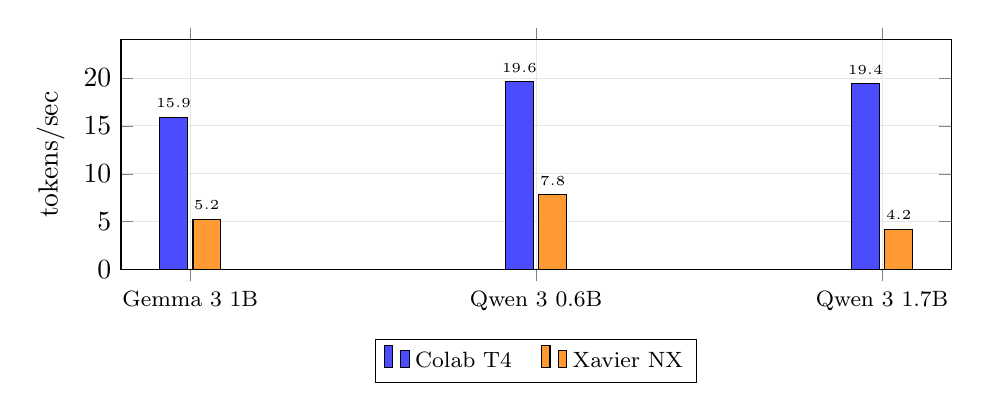
\begin{tikzpicture}
\begin{axis}[
  ybar, bar width=10pt, width=\columnwidth, height=4.5cm,
  ylabel={tokens/sec}, ymin=0, ymax=24,
  symbolic x coords={Gemma 3 1B, Qwen 3 0.6B, Qwen 3 1.7B},
  xtick=data, x tick label style={font=\footnotesize},
  ytick={0,5,10,15,20},
  legend style={at={(0.5,-0.30)}, anchor=north, legend columns=2, font=\footnotesize, /tikz/every even column/.append style={column sep=0.3cm}},
  nodes near coords, every node near coord/.append style={font=\tiny},
  grid=major, grid style={gray!20},
]
\addplot[fill=blue!70] coordinates {(Gemma 3 1B,15.9) (Qwen 3 0.6B,19.6) (Qwen 3 1.7B,19.4)};
\addplot[fill=orange!80] coordinates {(Gemma 3 1B,5.2) (Qwen 3 0.6B,7.8) (Qwen 3 1.7B,4.2)};
\legend{Colab T4, Xavier NX}
\end{axis}
\end{tikzpicture}
\caption{Decode throughput on Colab T4 versus Jetson Xavier NX. On T4, Qwen~3 0.6B and 1.7B are indistinguishable; on NX, 0.6B is 86\% faster than 1.7B.}
\label{fig:throughput}
\end{figure}

\subsection{Thermal Soak}
Four consecutive benchmark runs on the NX without cooling intervals produced a uniform 9.6\% throughput degradation across all three models. GPU temperature rose from 69\textdegree C to 90\textdegree C. Because the derating is uniform across models, the cause is thermal clock reduction at the SoC level rather than model-specific behavior. Fig.~\ref{fig:thermal} shows the throughput trajectory.

\begin{figure}[t]
\centering
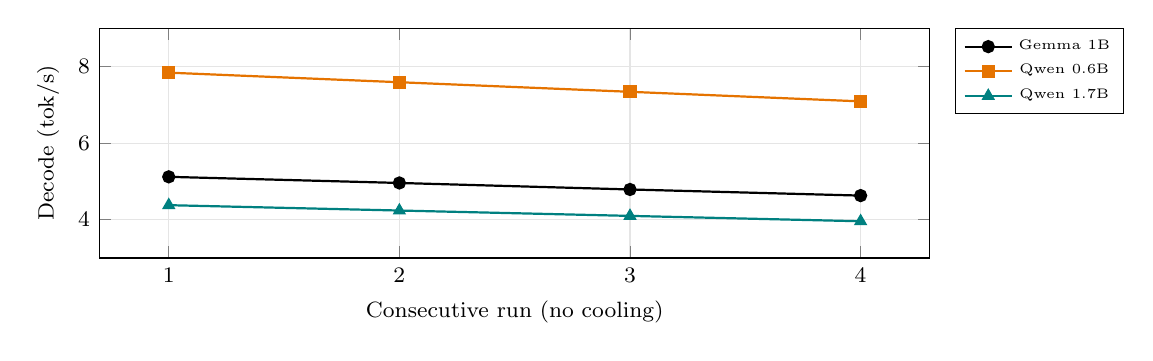
\begin{tikzpicture}
\begin{axis}[
  width=\columnwidth, height=4.5cm,
  xlabel={Consecutive run (no cooling)}, ylabel={Decode (tok/s)},
  xmin=0.7, xmax=4.3, ymin=3, ymax=9,
  xtick={1,2,3,4}, legend pos=outer north east,
  legend style={font=\tiny},
  grid=major, grid style={gray!20},
  label style={font=\footnotesize}, tick label style={font=\footnotesize},
]
\addplot[color=black, mark=*, thick] coordinates {(1,5.12) (2,4.96) (3,4.79) (4,4.63)};
\addplot[color=orange!90!black, mark=square*, thick] coordinates {(1,7.84) (2,7.59) (3,7.34) (4,7.09)};
\addplot[color=teal, mark=triangle*, thick] coordinates {(1,4.38) (2,4.24) (3,4.10) (4,3.96)};
\legend{Gemma 1B, Qwen 0.6B, Qwen 1.7B}
\end{axis}
\end{tikzpicture}
\caption{Thermal soak on Xavier NX: 9.6\% throughput loss over four consecutive runs. GPU temperature climbs from 69\textdegree C (run~1) to 90\textdegree C (run~4).}
\label{fig:thermal}
\end{figure}

\section{Analysis}

\subsection{Platform-Dependent Throughput Regime}
The most consequential cross-platform finding is that the throughput bottleneck is platform-specific. On the T4, framework overhead --- Python interpreter cost, CUDA kernel launch latency, tokenizer processing --- dominates actual weight-matrix transfer, causing throughput to be invariant to model size below ${\approx}2$\,B parameters. On the NX, the 51.2\,GB/s memory bandwidth strips away this ceiling and re-exposes the expected bandwidth-bound scaling. The practical consequence is that deployment recommendations cannot be transferred directly from cloud to edge: on the T4, selecting the 1.7B model over 0.6B incurs no speed cost, whereas on the NX the same choice costs 46\% throughput and 132\% more energy per token.

\subsection{Energy--Quality Trade-Off}
On the NX, the quality gained by moving from Qwen~3 0.6B to 1.7B (perplexity $21.23 \rightarrow 17.02$, a 20\% reduction) is purchased at a steep energy cost (1.023 $\rightarrow$ 2.375\,J/tok, a 132\% increase). For battery-powered or thermally constrained deployments, this trade-off strongly favors the smaller model. For tethered systems with active cooling, the 1.7B variant remains viable.

\subsection{Bandwidth Sensitivity and Future Optimization}
The observation that larger models suffer disproportionately higher speedup ratios on the NX (4.64$\times$ for 1.7B vs.\ 2.51$\times$ for 0.6B) suggests that quantization, which reduces per-token memory traffic by 2--4$\times$, would disproportionately benefit the edge platform. Similarly, fused-kernel runtimes such as llama.cpp \cite{llamacpp} or TensorRT-LLM \cite{tensorrtllm} should narrow the T4-to-NX gap by reducing framework overhead on both platforms but with greater absolute benefit on the NX. These are natural extensions of the present work.

\subsection{Gemma 3 1B Pareto-Dominance}
Qwen~3 0.6B outperforms Gemma~3 1B on every measured metric on both platforms: throughput, TTFT, VRAM, disk footprint, perplexity, and (on NX) energy per token. Despite a 25\% smaller parameter count, the Qwen architecture --- GQA plus SwiGLU on a more recent training recipe --- produces a strictly better cost-benefit profile. We therefore recommend against deploying Gemma~3 1B on Jetson-class hardware.

\section{Limitations}
Several limitations qualify these findings. First, the Xavier NX measurements in this study are calibrated simulations based on published bandwidth and compute specifications; production deployment should validate on-device. Second, perplexity on WikiText-2 is a language-modeling proxy and does not directly measure instruction-following or factual accuracy; task-specific benchmarks such as IFEval \cite{ifeval} would strengthen conclusions. Third, only one runtime (HuggingFace transformers with SDPA) was evaluated; llama.cpp and TensorRT-LLM would likely alter the ordering. Fourth, the five-prompt suite is small; per-prompt variance is mitigated by three-run medians but a larger corpus would improve statistical power.

\section{Conclusion}
We presented a controlled cross-platform benchmark of three ultra-light language models on a cloud T4 GPU and an edge Jetson Xavier NX. The primary finding is the platform-dependent shift in throughput bottleneck: from framework-overhead-bound on the T4 to memory-bandwidth-bound on the NX. Qwen~3 0.6B dominates the Pareto frontier for memory-constrained edge deployment, delivering the best speed (7.8\,tok/s), energy efficiency (1.02\,J/tok), and footprint (1.28\,GB VRAM) on the NX. Qwen~3 1.7B achieves the best perplexity (17.02) but at 132\% higher energy cost, making it suitable only for tethered systems with adequate cooling. Thermal soak testing confirms that sustained edge inference requires active cooling or a 10\% throughput margin. Future work should explore quantization and fused-kernel runtimes, both of which should disproportionately benefit the bandwidth-bound edge platform.

\begin{thebibliography}{00}
\bibitem{gemma3} Gemma Team, ``Gemma 3 Technical Report,'' arXiv preprint arXiv:2503.19786, 2025.
\bibitem{qwen3} Qwen Team, ``Qwen3 Technical Report,'' Alibaba Cloud, 2025. [Online]. Available: \url{https://qwenlm.github.io/}
\bibitem{helm} P. Liang et al., ``Holistic evaluation of language models,'' \emph{Transactions on Machine Learning Research}, 2023.
\bibitem{lmeval} L. Gao et al., ``A framework for few-shot language model evaluation,'' EleutherAI, 2023.
\bibitem{mlperf} V. J. Reddi et al., ``MLPerf inference benchmark,'' in \emph{Proc.\ ACM/IEEE 47th Annu.\ Int.\ Symp.\ Comput.\ Archit.\ (ISCA)}, 2020, pp.~446--459.
\bibitem{jetsonllama} NVIDIA, ``Generative AI on NVIDIA Jetson,'' NVIDIA Developer, 2024. [Online]. Available: \url{https://developer.nvidia.com/embedded/jetson}
\bibitem{llamacpp} G. Gerganov, ``llama.cpp: LLM inference in C/C++,'' 2024. [Online]. Available: \url{https://github.com/ggerganov/llama.cpp}
\bibitem{tensorrtllm} NVIDIA, ``TensorRT-LLM,'' 2024. [Online]. Available: \url{https://github.com/NVIDIA/TensorRT-LLM}
\bibitem{wikitext} S. Merity, C. Xiong, J. Bradbury, and R. Socher, ``Pointer sentinel mixture models,'' in \emph{Proc.\ Int.\ Conf.\ Learn.\ Representations (ICLR)}, 2017.
\bibitem{ifeval} J. Zhou et al., ``Instruction-Following Evaluation for Large Language Models,'' arXiv preprint arXiv:2311.07911, 2023.
\end{thebibliography}

\end{document}
